\documentclass[tikz,border=4pt]{standalone}
\usepackage{amsmath}
\definecolor{curveblue}{HTML}{245C86}
\begin{document}
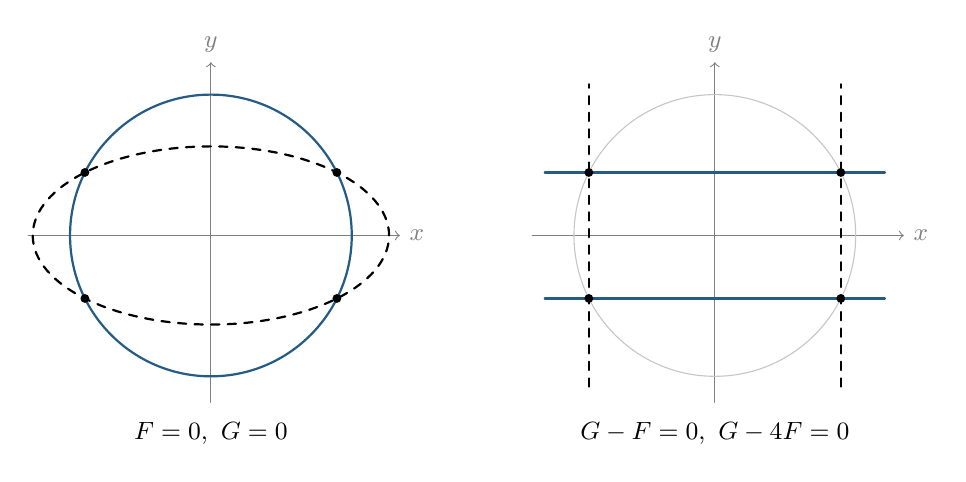
\begin{tikzpicture}[font=\small,line cap=round,scale=.8]
\begin{scope}
\draw[gray,->](-2.9,0)--(3,0)node[right]{$x$};
\draw[gray,->](0,-2.65)--(0,2.75)node[above]{$y$};
\draw[curveblue,thick](0,0)circle({sqrt(5)});
\draw[thick,dashed](0,0)ellipse[x radius={sqrt(8)},y radius={sqrt(2)}];
\foreach \x in {-2,2}{\foreach \y in {-1,1}{\fill(\x,\y)circle(2pt);}}
\node at(0,-3.15){$F=0,\ G=0$};
\end{scope}
\begin{scope}[shift={(8,0)}]
\draw[gray,->](-2.9,0)--(3,0)node[right]{$x$};
\draw[gray,->](0,-2.65)--(0,2.75)node[above]{$y$};
\draw[gray!45](0,0)circle({sqrt(5)});
\draw[curveblue,thick](-2.7,1)--(2.7,1) (-2.7,-1)--(2.7,-1);
\draw[thick,dashed](-2,-2.4)--(-2,2.4) (2,-2.4)--(2,2.4);
\foreach \x in {-2,2}{\foreach \y in {-1,1}{\fill(\x,\y)circle(2pt);}}
\node at(0,-3.15){$G-F=0,\ G-4F=0$};
\end{scope}
\end{tikzpicture}
\end{document}
